%==============================================================================
%  MATH 231 -- Linear Algebra I (Queens College, Fall 2026)
%  MIDTERM 2, PRACTICE EXAM -- built from Homework 3 and Homework 4
%
%  SCOPE.  Matrix Unit, Parts 1-10 (lectures 1-10; Part 11, Gram-Schmidt and
%  QR, is not on Midterm 2), with the emphasis on the problems of
%     homework/MATH231_homework_3.tex   Parts A-D
%     homework/MATH231_homework_4.tex   Parts A-F (A.4, linear and affine maps,
%                                       left out: it is not a Part 1-10 lecture)
%  Every question is a close relative of a homework problem with new numbers,
%  not a verbatim copy.  Programming is not assessed on exams (syllabus S7).
%
%  FORMAT.  Same layout as Midterm 1 (exams/midterm1/MATH231_midterm_1.tex),
%  with two changes the instructor asked for: there is no cover page with a
%  grading table (the title, the name line and Question 1 share page 1), and
%  no question or part carries points.  20 questions, numbered straight
%  through, with no section headings and no true/false:
%     Multiple choice   Question   1       (seven parts, circle all that apply)
%     Computation       Questions  2-16
%     Proofs            Questions 17-20
%
%  SOURCES (question -> homework problem):
%     Q1  mixed: shapes (HW3 D.1), laws (HW3 D, M1-M6), D10, orthogonal
%         matrices (HW4 A.1(c)), projections (HW4 B), rank-nullity (HW4 D.1),
%         least squares (HW4 F)
%     Q2  HW3 A.1-A.3       Q8  HW4 A.2-A.3      Q14 HW4 E.1-E.2
%     Q3  HW3 B.1-B.3       Q9  HW4 B.1          Q15 HW4 E.3, D.2(d)
%     Q4  HW3 C.1-C.2       Q10 HW4 B.2-B.3      Q16 HW4 F.1-F.2
%     Q5  HW3 D.1-D.2, D.4  Q11 HW4 C.1, C.3(a)  Q17 HW3 B.3, HW4 C.3(b)
%     Q6  HW3 D.3, D.5      Q12 HW4 C.2-C.3      Q18 HW3 C.2(d), D.4(d), D.5(c)
%     Q7  HW4 A.1           Q13 HW4 D.1          Q19 HW4 A.3(a), B.2(a)-(b)
%                                                Q20 HW4 D.2(a)-(b), E.3(d)-(e)
%
%  CALCULATOR-FREE.  Every number was checked with sympy; all answers are exact
%  and small.  There is no answer key in this file.  The \sol, \yn[Y], \correct
%  and \blank[answer] machinery of Midterm 1 is kept in the preamble, so a key
%  can be added later exactly as on Midterm 1.
%
%  \contd prints the current question number, so moving a question needs no
%  renumbering by hand.
%
%  Compile with tectonic (or pdflatex; standard TeX Live packages only; uses
%  tikz for the grids in Questions 7 and 16).
%==============================================================================

\documentclass[11pt]{article}

\usepackage[margin=1in,headheight=14pt]{geometry}
\usepackage{amsmath,amssymb}
\usepackage[dvipsnames]{xcolor}
\usepackage{enumitem}
\usepackage{booktabs}
\usepackage{array}
\usepackage[hidelinks]{hyperref}
\usepackage{titlesec}
\usepackage{needspace}
\usepackage{colortbl}
\usepackage{fancyhdr}
\usepackage{tikz}
\usetikzlibrary{arrows.meta}

%---------------------------------------------------------------- solutions --
% Same switch as Midterm 1: a wrapper that defines \solutionsmode as 1 and
% \inputs this file turns on every \sol box, red circle and red blank answer.
\providecommand{\solutionsmode}{0}
\newif\ifsolutions
\if1\solutionsmode\solutionstrue\fi

\makeatletter
\newcommand{\sol}[1]{\ifsolutions\par\nointerlineskip
  \moveright\@totalleftmargin\vbox to 0pt{\hsize=\linewidth\vskip 3pt
    \noindent\fcolorbox{red}{white}{\parbox{\dimexpr\linewidth-2\fboxsep-2\fboxrule\relax}%
      {\color{red}\small\setlength{\parskip}{3pt}#1}}\par\vss}\fi}

\newcommand{\solcirc}[1]{\tikz[baseline=(sc.base)]{\node[inner sep=0pt](sc){#1};
  \draw[red,thick,overlay,rounded corners=3pt]
    ([shift={(-2.5pt,-2.5pt)}]sc.south west) rectangle
    ([shift={(2.5pt,2.5pt)}]sc.north east);}}
\newcommand{\solmark}[1]{\ifsolutions\solcirc{#1}\else#1\fi}
\newcommand{\correct}{}
\newcommand{\lab}[1]{\ifsolutions
  \edef\lab@tmp{\noexpand\in@{#1}{\correct}}\lab@tmp
  \ifin@\solcirc{(#1)}\else(#1)\fi
  \else(#1)\fi}
\makeatother

%------------------------------------------------------------------ style ----
% A running header on every page but the first (\maketitle gives page 1 the
% plain style: a page number and no header).
\pagestyle{fancy}
\fancyhf{}
\fancyhead[C]{\small\sffamily MATH 231 -- Linear Algebra I (Fall 2026)
  \quad|\quad Midterm 2 Practice\ifsolutions\ \textcolor{red}{Solutions}\fi{} \quad|\quad Kevin Bedoya}
\fancyfoot[C]{\thepage}
\renewcommand{\headrulewidth}{0.4pt}

\titleformat{\section}{\large\bfseries\sffamily\color{RoyalBlue}}{}{0em}{}
\titlespacing*{\section}{0pt}{0pt}{7pt}

% Keeps long inline formulas from pushing a line into the margin.
\setlength{\emergencystretch}{3em}

% The question heading is a line of its own, so that part (i) -- or the
% opening sentence -- always starts below it.  Same environment as Midterm 1,
% without the points at the right end of the line.
\makeatletter
\newcounter{prob}
% Usage: \begin{prob}[title].
\newenvironment{prob}[1][]
  {\par\addvspace{12pt plus 4pt minus 4pt}%
   \needspace{4\baselineskip}%
   \refstepcounter{prob}%
   \noindent\textbf{Question~\theprob}%
   \if\relax\detokenize{#1}\relax\else\ (#1)\fi\textbf{.}%
   \par\nobreak\@afterindentfalse\@afterheading}
  {\par}
\makeatother

\newcommand{\hint}[1]{\par\smallskip\noindent
  {\small\sffamily\textcolor{RoyalBlue}{\textbf{Hint.}}\ #1}\par\smallskip}

% A question that runs onto a second page continues under this line.
\newcommand{\contd}{\newpage\noindent
  {\small\sffamily\color{gray}Question~\theprob, continued}\par\medskip}

% Yes or no: the question on the left, the two words to circle on the right of
% its first line.  The optional argument, Y or N, is the answer.
\newcommand{\yn}[2][]{\parbox[t]{\dimexpr\linewidth-7em}{#2}%
  \hfill\textsf{\textbf{\ynopt{Y}{#1}{Yes}}\qquad\textbf{\ynopt{N}{#1}{No}}}}
\newcommand{\ynopt}[3]{\ifsolutions\def\ynA{#1}\def\ynB{#2}%
  \ifx\ynA\ynB\solcirc{#3}\else#3\fi\else#3\fi}

% A line to write an answer on.  The optional argument is its answer, printed
% in red on the line in the solutions build only.
\newcommand{\blank}[2][]{\ifsolutions\if\relax\detokenize{#1}\relax\else
  \makebox[0pt][l]{\hspace{4pt}\raisebox{3pt}{\color{red}#1}}\fi\fi
  \rule[-2pt]{#2}{0.4pt}}

% list styles used throughout
\newlist{romparts}{enumerate}{1}
\setlist[romparts]{leftmargin=2.6em,label=\textbf{(\roman*)},itemsep=0pt,
                   topsep=6pt}

% Multiple choice: long options one per line, short ones three to a row.
\newlist{opts}{enumerate}{1}
\setlist[opts]{leftmargin=*,label=(\alph*),itemsep=2pt,topsep=4pt}
\newcommand{\threech}[5]{\par\smallskip\noindent
  \begin{tabular}{@{}*{3}{>{\raggedright\arraybackslash}p{0.3\linewidth}}@{}}
  \lab{a}\ #1 & \lab{b}\ #2 & \lab{c}\ #3 \\[4pt]
  \lab{d}\ #4 & \lab{e}\ #5 &
  \end{tabular}\par}

% The words to circle in Question 2(vii).
\newcommand{\patternwords}{{\sffamily\setlength{\tabcolsep}{0.9em}%
  \begin{tabular}[t]{@{}llll@{}}
  square & rectangular & diagonal & identity \\[3pt]
  upper triangular & lower triangular & tridiagonal & symmetric
  \end{tabular}}}

%------------------------------------------------------------- tikz helpers --
\tikzset{
  vecarr/.style   = {-{Stealth[length=2.6mm,width=2.0mm]},very thick},
  axisline/.style = {->,gray!75,thin}
}

%--------------------------------------------------------------- notation ----
\newcommand{\R}{\mathbb{R}}
\newcommand{\vc}[1]{\mathbf{#1}}
\newcommand{\mt}[1]{\mathbf{#1}}
\newcommand{\T}{^{\mathsf{T}}}
\newcommand{\one}{\mathbf{1}}
\newcommand{\norm}[1]{\lVert #1\rVert}
\newcommand{\colsp}[1]{\operatorname{col}[#1]}
\newcommand{\nullsp}[1]{\operatorname{null}[#1]}
\newcommand{\xh}{\hat{\vc{x}}}
\DeclareMathOperator{\spanop}{span}
\DeclareMathOperator{\rank}{rank}
\DeclareMathOperator{\nullity}{nullity}
\DeclareMathOperator{\tr}{tr}
\DeclareMathOperator{\diagop}{diag}
\DeclareMathOperator{\adj}{adj}

\title{\vspace{-1.2cm}\textbf{\sffamily MATH 231 -- Linear Algebra I (Fall 2026)}\\[4pt]
       {\large\sffamily Midterm 2 \textbullet\ Practice Exam\ifsolutions\ \textbullet\ \textcolor{red}{Solutions}\fi}\\[2pt]
       {\normalsize\sffamily Kiely Hall 326 \textbullet\
        Instructor: Kevin Bedoya}}
\author{}
\date{}

\begin{document}
\maketitle
\vspace{-1.4cm}

\begin{center}
\large\sffamily Full name: \rule{6.5cm}{0.4pt}\hspace{1cm}%
CUNY ID: \rule{3.8cm}{0.4pt}
\end{center}
\medskip

% The notation the exam states.  \boldmath bolds the math too.
\noindent{\bfseries\boldmath A vector $\vc{x}\in\R^{n}$ is a column. A bracket
written across the line is a row, so a column written across the line carries a
transpose: $[\,3,\,1\,]\in\R^{1\times2}$ is a row and
$[\,3,\,1\,]\T\in\R^{2}$ is a column. For a matrix $\mt{A}$,
$\colsp{\mt{A}}$ and $\nullsp{\mt{A}}$ denote its column space and its null
space.}
\par\medskip

%------------------------------------------------------------------------------
\begin{prob}[Multiple choice]
\begin{romparts}
  \item Let $\mt{A}\in\R^{2\times3}$, $\mt{B}\in\R^{3\times3}$ and
        $\vc{c}\in\R^{3}$. Circle all of the following products that are
        defined:
        \threech{$\mt{A}\mt{B}$}
                {$\mt{B}\mt{A}$}
                {$\mt{A}\vc{c}$}
                {$\vc{c}\T\mt{B}$}
                {$\vc{c}\,\mt{A}$}
        \vspace{0.5cm}
  \item Let $\mt{A},\mt{B},\mt{C}$ be $n\times n$ matrices. Circle all that are
        \textbf{always} true:
        \par\smallskip\noindent
        \begin{tabular}{@{}*{2}{>{\raggedright\arraybackslash}p{0.46\linewidth}}@{}}
        \lab{a}\ $(\mt{A}\mt{B})\T=\mt{A}\T\mt{B}\T$ &
        \lab{b}\ $(\mt{A}\mt{B})\T=\mt{B}\T\mt{A}\T$ \\[4pt]
        \lab{c}\ $\mt{A}\mt{B}=\mt{B}\mt{A}$ &
        \lab{d}\ $\mt{A}(\mt{B}+\mt{C})=\mt{A}\mt{B}+\mt{A}\mt{C}$ \\[4pt]
        \lab{e}\ $(\mt{A}+\mt{B})\T=\mt{A}\T+\mt{B}\T$ &
        \lab{f}\ $\tr(\mt{A}\mt{B})=\tr(\mt{A})\tr(\mt{B})$
        \end{tabular}
        \vspace{0.5cm}
  \item Let $\mt{A}\in\R^{n\times n}$ with $\det\mt{A}\neq0$. Circle all that
        must be true:
        \begin{opts}
          \item[\lab{a}] $\rank\mt{A}=n$.
          \item[\lab{b}] $\nullsp{\mt{A}}=\{\vc{0}\}$.
          \item[\lab{c}] For every $\vc{b}\in\R^{n}$, the system
                $\mt{A}\vc{x}=\vc{b}$ has exactly one solution.
          \item[\lab{d}] $\mt{A}$ is symmetric.
          \item[\lab{e}] $\det(\mt{A}^{-1})=\det\mt{A}$.
        \end{opts}
        \vspace{0.5cm}
  \item Circle all of the following matrices that are orthogonal:
        % \threech, with more room between its rows for the matrices.
        \par\smallskip\noindent
        \begin{tabular}{@{}*{3}{>{\raggedright\arraybackslash}p{0.3\linewidth}}@{}}
        \lab{a}\ $\begin{bmatrix}0&1\\1&0\end{bmatrix}$ &
        \lab{b}\ $\begin{bmatrix}1&1\\0&1\end{bmatrix}$ &
        \lab{c}\ $\dfrac{1}{\sqrt2}\begin{bmatrix}1&-1\\1&1\end{bmatrix}$ \\[14pt]
        \lab{d}\ $\begin{bmatrix}2&0\\0&\tfrac12\end{bmatrix}$ &
        \lab{e}\ $\begin{bmatrix}-1&0\\0&-1\end{bmatrix}$ &
        \end{tabular}
\end{romparts}
% Page 1 also carries the title and the name line, so Question 1 runs onto
% page 2.
\contd
\begin{romparts}[resume]
  \item Let $\mt{P}\in\R^{n\times n}$ with $\mt{P}^{2}=\mt{P}$, $\mt{P}\T=\mt{P}$
        and $\mt{P}\neq\mt{I}$. Circle all that must be true:
        \begin{opts}
          \item[\lab{a}] $(\mt{I}-\mt{P})^{2}=\mt{I}-\mt{P}$.
          \item[\lab{b}] $\mt{P}$ is invertible.
          \item[\lab{c}] $\det\mt{P}=0$.
          \item[\lab{d}] $(2\mt{P}-\mt{I})\T(2\mt{P}-\mt{I})=\mt{I}$.
          \item[\lab{e}] For every $\vc{v}\in\R^{n}$, $\mt{P}\vc{v}$ is
                orthogonal to $\vc{v}-\mt{P}\vc{v}$.
        \end{opts}
        \vspace{0.5cm}
  \item Let $\mt{A}\in\R^{4\times6}$ with $\rank\mt{A}=4$. Circle all that must
        be true:
        \begin{opts}
          \item[\lab{a}] $\nullity\mt{A}=2$.
          \item[\lab{b}] $\mt{A}$ has full row rank.
          \item[\lab{c}] $\mt{A}\vc{x}=\vc{b}$ is consistent for every
                $\vc{b}\in\R^{4}$.
          \item[\lab{d}] The columns of $\mt{A}$ are linearly independent.
          \item[\lab{e}] $\nullsp{\mt{A}\T}=\{\vc{0}\}$.
        \end{opts}
        \vspace{0.5cm}
  \item Let $\mt{A}\in\R^{m\times n}$ and $\vc{b}\in\R^{m}$, and let $\xh$ be a
        least-squares solution of $\mt{A}\vc{x}=\vc{b}$. Circle all that must be
        true:
        \begin{opts}
          \item[\lab{a}] $\mt{A}\T\mt{A}\,\xh=\mt{A}\T\vc{b}$.
          \item[\lab{b}] $\vc{b}-\mt{A}\xh$ is orthogonal to every column of
                $\mt{A}$.
          \item[\lab{c}] $\mt{A}\xh=\vc{b}$.
          \item[\lab{d}] If $\mt{A}$ has full column rank, then $\xh$ is unique.
          \item[\lab{e}] $\norm{\mt{A}\xh-\vc{b}}\le\norm{\mt{A}\vc{x}-\vc{b}}$
                for every $\vc{x}\in\R^{n}$.
        \end{opts}
\end{romparts}
\end{prob}

\newpage
%------------------------------------------------------------------------------
\begin{prob}[Reading and building a matrix]
Let
\[
  \mt{A}=\begin{bmatrix}3&-2&0&8\\5&7&-4&2\\0&1&6&-3\end{bmatrix}.
\]
\begin{romparts}
  \item The dimensions of $\mt{A}$ are \blank{1.2cm} $\times$ \blank{1.2cm},
        and $\mt{A}$ has \blank{1.2cm} entries.
        \vspace{\stretch{0.5}}
  \item $a_{23}=$ \blank{1.6cm} \qquad $a_{32}=$ \blank{1.6cm} \qquad
        $a_{14}=$ \blank{1.6cm}
        \vspace{\stretch{0.5}}
  \item \yn{Does the entry $a_{41}$ of $\mt{A}$ exist? (circle one) Explain
        why.}
        \vspace{\stretch{0.8}}
  \item Write row $2$ of $\mt{A}$ as a row vector, and column $3$ of $\mt{A}$ as
        a column vector.
        \vspace{\stretch{1.2}}
  \item Write out the matrix $\mt{B}\in\R^{4\times4}$ with $b_{ij}=i+j$ if
        $i\le j$, and $b_{ij}=0$ if $i>j$.
        \vspace{\stretch{1.6}}
  \item Write out the matrix $\mt{C}\in\R^{4\times4}$ with $c_{ij}=1$ if
        $\lvert i-j\rvert\le1$, and $c_{ij}=0$ otherwise.
        \vspace{\stretch{1.6}}
  \item For each of $\mt{B}$ and $\mt{C}$, circle every word that describes it.
        \par\medskip\noindent
        $\mt{B}$:\quad \patternwords
        \par\bigskip\noindent
        $\mt{C}$:\quad \patternwords
        \vspace{\stretch{0.3}}
\end{romparts}
\end{prob}

\newpage
%------------------------------------------------------------------------------
\begin{prob}[Adding, scaling, and the transpose]
Let
\[
  \mt{A}=\begin{bmatrix}2&-1&3\\0&4&-2\end{bmatrix},
  \qquad
  \mt{B}=\begin{bmatrix}0&5&-1\\2&-2&0\end{bmatrix},
  \qquad
  \mt{C}=\begin{bmatrix}2&1\\0&-3\\4&1\end{bmatrix}.
\]
\begin{romparts}
  \item Compute $2\mt{A}-3\mt{B}$.
        \vspace{\stretch{1}}
  \item \yn{Is $\mt{A}+\mt{C}$ defined? (circle one) Explain why.}
        \vspace{\stretch{0.7}}
  \item Compute $\mt{A}+\mt{C}\T$.
        \vspace{\stretch{1}}
  \item Find the matrix $\mt{X}$ with $3\mt{X}-\mt{B}=\mt{X}+\mt{A}$. Solve for
        $\mt{X}$ first, and only then substitute.
        \vspace{\stretch{1.4}}
  \item Find every $x$, $y$ and $z$ for which
        $\begin{bmatrix}2&x&-1\\3&0&y\\z&5&4\end{bmatrix}$ is symmetric.
        \vspace{\stretch{1}}
  \item A square matrix $\mt{K}$ is \textbf{skew-symmetric} if
        $\mt{K}\T=-\mt{K}$. Write
        \[
          \mt{M}=\begin{bmatrix}2&3&-1\\1&0&4\\5&-2&1\end{bmatrix}
        \]
        as the sum of a symmetric matrix and a skew-symmetric matrix.
        \hint{Compute $\tfrac12(\mt{M}+\mt{M}\T)$ and
        $\tfrac12(\mt{M}-\mt{M}\T)$.}
        \vspace{\stretch{2}}
\end{romparts}
\end{prob}

\newpage
%------------------------------------------------------------------------------
\begin{prob}[Inner and outer products]
Let $\vc{u}=[\,2,\,-1,\,2\,]\T$ and $\vc{v}=[\,1,\,3,\,-2\,]\T$.
\begin{romparts}
  \item Compute $\vc{u}\T\vc{v}$, and give its shape.
        \vspace{\stretch{1}}
  \item Use $\vc{u}\T\vc{u}$ to compute $\norm{\vc{u}}$.
        \vspace{\stretch{0.8}}
  \item Compute $\vc{u}\vc{v}\T$, and give its shape.
        \vspace{\stretch{1.4}}
  \item Compute $\tr(\vc{u}\vc{v}\T)$, and compare it with your answer to (i).
        \vspace{\stretch{0.8}}
  \item The matrix $\begin{bmatrix}3&-6&9\\-1&2&-3\end{bmatrix}$ is an outer
        product $\vc{x}\vc{y}\T$. Find $\vc{x}\in\R^{2}$ and $\vc{y}\in\R^{3}$,
        and check your answer by multiplying out.
        \vspace{\stretch{1.4}}
  \item \yn{Is $\begin{bmatrix}1&2\\2&3\end{bmatrix}$ an outer product
        $\vc{x}\vc{y}\T$ of two vectors $\vc{x},\vc{y}\in\R^{2}$? (circle one)
        Explain why.}
        \vspace{\stretch{1.4}}
\end{romparts}
\end{prob}

\newpage
%------------------------------------------------------------------------------
\begin{prob}[Matrix multiplication]
\begin{romparts}
  \item Let $\mt{A}\in\R^{3\times2}$, $\mt{B}\in\R^{2\times4}$,
        $\mt{C}\in\R^{4\times1}$ and $\mt{D}\in\R^{1\times3}$. Under each
        product, write its shape, or write \emph{undefined}.
        \par\medskip
        \begin{center}
        \renewcommand{\arraystretch}{1.3}
        \begin{tabular}{|*{8}{>{\centering\arraybackslash}p{1.35cm}|}}
        \hline
        $\mt{A}\mt{B}$ & $\mt{B}\mt{A}$ & $\mt{B}\mt{C}$ & $\mt{D}\mt{A}$ &
        $\mt{C}\mt{D}$ & $\mt{A}\mt{B}\mt{C}$ & $\mt{D}\mt{A}\mt{B}$ &
        $\mt{C}\T\mt{C}$ \\ \hline
        \rule{0pt}{0.9cm} & & & & & & & \\ \hline
        \end{tabular}
        \end{center}
        \vspace{\stretch{0.4}}
  \item Let $\mt{E}=\begin{bmatrix}1&2\\-1&3\end{bmatrix}$ and
        $\mt{F}=\begin{bmatrix}2&0\\1&-1\end{bmatrix}$. Compute $\mt{E}\mt{F}$
        and $\mt{F}\mt{E}$.
        \vspace{\stretch{1.5}}
        \par\noindent
        \yn{Is $\mt{E}\mt{F}=\mt{F}\mt{E}$? (circle one)}
        \vspace{\stretch{0.3}}
  \item Let $\mt{G}=\begin{bmatrix}1&-1&2\\0&3&1\end{bmatrix}$ and
        $\mt{H}=\begin{bmatrix}2&1\\0&-1\\1&1\end{bmatrix}$. Compute
        $\mt{G}\mt{H}$ and $\mt{H}\mt{G}$.
        \vspace{\stretch{2}}
\end{romparts}
\contd
\begin{romparts}[resume]
  \item Let $\mt{A}=\begin{bmatrix}1&2\\2&4\end{bmatrix}$ and
        $\mt{B}=\begin{bmatrix}-2&6\\1&-3\end{bmatrix}$. Compute $\mt{A}\mt{B}$
        and $\mt{B}\mt{A}$.
        \vspace{\stretch{1.5}}
        \par\noindent
        \yn{For real numbers, $ab=0$ forces $a=0$ or $b=0$. For matrices, does
        $\mt{A}\mt{B}=\mt{0}$ force $\mt{A}=\mt{0}$ or $\mt{B}=\mt{0}$?
        (circle one)}
        \vspace{\stretch{0.5}}
  \item Let $\mt{N}=\begin{bmatrix}0&2&0\\0&0&3\\0&0&0\end{bmatrix}$. Compute
        $\mt{N}^{2}$ and $\mt{N}^{3}$.
        \vspace{\stretch{1.5}}
  \item Let $\mt{S}=\begin{bmatrix}1&2\\0&1\end{bmatrix}$. Compute
        $\mt{S}^{2}$ and $\mt{S}^{3}$, and guess a formula for $\mt{S}^{n}$.
        \vspace{\stretch{1.5}}
\end{romparts}
\end{prob}

\newpage
%------------------------------------------------------------------------------
\begin{prob}[Matrix--vector products, two ways]
\begin{romparts}
  \item Compute
        $\begin{bmatrix}2&1&-1\\0&3&4\end{bmatrix}\begin{bmatrix}3\\-2\\1\end{bmatrix}$
        twice: by rows, and by columns.
        \vspace{\stretch{1.4}}
  \item Compute
        $\begin{bmatrix}1&2&3\\2&3&4\\3&4&5\end{bmatrix}\begin{bmatrix}1\\-2\\1\end{bmatrix}$.
        \vspace{\stretch{0.8}}
        \par\noindent
        \yn{Are the columns of this $3\times3$ matrix linearly independent?
        (circle one) Explain why, using the product you computed.}
        \vspace{\stretch{1}}
  \item Let $\mt{A}=\begin{bmatrix}2&0&1\\1&-1&3\\4&2&0\end{bmatrix}$, with
        columns $\vc{a}_1,\vc{a}_2,\vc{a}_3$. Use the column reading, and no
        equation solving, to find a vector $\vc{x}$ with
        $\mt{A}\vc{x}=\vc{a}_3$, and a vector $\vc{x}$ with
        $\mt{A}\vc{x}=2\vc{a}_1-\vc{a}_2$.
        \vspace{\stretch{1.2}}
  \item With $\mt{A}$ from (iii), \
        $\vc{e}_2\T\mt{A}\,\vc{e}_3=$ \blank{2cm}
        \vspace{\stretch{0.5}}
  \item Find the $2\times2$ matrix $\mt{M}$ with
        $\mt{M}[\,1,\,0\,]\T=[\,4,\,-1\,]\T$ and
        $\mt{M}[\,0,\,1\,]\T=[\,2,\,3\,]\T$. Then compute
        $\mt{M}[\,1,\,-2\,]\T$ by the column reading.
        \vspace{\stretch{1.2}}
  \item Let $\mt{D}=\diagop(3,-1,2)$, the $3\times3$ diagonal matrix with
        diagonal entries $3,-1,2$, and let
        $\mt{G}=\begin{bmatrix}1&2&3\\4&5&6\\7&8&9\end{bmatrix}$. Compute
        $\mt{D}\mt{G}$ and $\mt{G}\mt{D}$. In each product, what happened to the
        rows or the columns of $\mt{G}$?
        \vspace{\stretch{1.8}}
\end{romparts}
\end{prob}

\newpage
%------------------------------------------------------------------------------
\begin{prob}[Moving the plane]
Let $S$ be the unit square with corners $(0,0)$, $(1,0)$, $(1,1)$, $(0,1)$,
taken in that order, and let
\[
  \mt{V}_S=\begin{bmatrix}0&1&1&0\\0&0&1&1\end{bmatrix},
  \qquad
  \mt{M}=\begin{bmatrix}1&2\\0&1\end{bmatrix}.
\]
\par\smallskip\noindent
% Parts (i)-(iii) on the left, the axes they draw on at the right.
\begin{minipage}[t]{0.55\textwidth}
\vspace{0pt}
\begin{romparts}
  \item Compute $\mt{M}\mt{V}_S$. Then draw $S$ and its image under $\mt{M}$ on
        the axes at right.
        \par\vspace{2.6cm}
  \item What kind of motion is $\mt{M}$? Your answer should be a single word.
        \par\medskip\blank{4cm}
        \par\vspace{0.8cm}
  \item The area of the image of $S$ is \blank{1.5cm}, and
        $\det\mt{M}=$ \blank{1.5cm}.
\end{romparts}
\end{minipage}\hfill
\begin{minipage}[t]{0.42\textwidth}
\vspace{0pt}
\centering
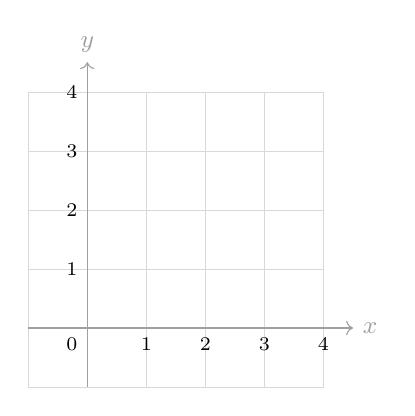
\begin{tikzpicture}[scale=0.75]
  \draw[step=1,gray!30,very thin] (-1,-1) grid (4,4);
  \draw[axisline] (-1,0) -- (4.5,0) node[right,font=\small]{$x$};
  \draw[axisline] (0,-1) -- (0,4.5) node[above,font=\small]{$y$};
  \foreach \i in {1,...,4}{
    \node[below,font=\scriptsize] at (\i,0) {$\i$};
    \node[left,font=\scriptsize]  at (0,\i) {$\i$};}
  \node[below left,font=\scriptsize] at (0,0) {$0$};
\end{tikzpicture}
\end{minipage}
\par\vspace{0.8cm}
\begin{romparts}[start=4]
  \item Find the $2\times2$ matrix that moves the triangle with corners
        $(0,0)$, $(1,0)$, $(0,1)$ onto the triangle with corners $(0,0)$,
        $(2,1)$, $(-1,3)$, sending $(1,0)$ to $(2,1)$ and $(0,1)$ to $(-1,3)$.
        Then use a determinant to find the area of the second triangle.
        \vspace{\stretch{1.6}}
  \item \yn{Is there a $2\times2$ matrix that moves the triangle with corners
        $(0,0)$, $(1,0)$, $(0,1)$ onto the triangle with corners $(2,1)$,
        $(3,1)$, $(2,2)$? (circle one) Explain why.}
        \vspace{\stretch{1}}
  \item Write a $3\times3$ matrix, in homogeneous coordinates, that moves the
        triangle with corners $(0,0)$, $(1,0)$, $(0,1)$ onto the triangle with
        corners $(2,1)$, $(3,1)$, $(2,2)$.
        \vspace{\stretch{1.2}}
\end{romparts}
\end{prob}

\newpage
%------------------------------------------------------------------------------
\begin{prob}[Rotations, reflections, and orthogonal matrices]
Let
\[
  \mt{R}=\begin{bmatrix}0&-1\\1&0\end{bmatrix},
  \qquad
  \mt{F}=\begin{bmatrix}1&0\\0&-1\end{bmatrix},
\]
so that $\mt{R}$ is the quarter turn counterclockwise and $\mt{F}$ is the
reflection across the $x$-axis.
\begin{romparts}
  \item Compute $\mt{F}\mt{R}$ and $\mt{R}\mt{F}$.
        \vspace{\stretch{1.2}}
        \par\noindent
        \yn{Is $\mt{F}\mt{R}=\mt{R}\mt{F}$? (circle one)}
        \vspace{\stretch{0.3}}
  \item Each of $\mt{F}\mt{R}$ and $\mt{R}\mt{F}$ is a reflection. Give the line
        that each one reflects across.
        \par\medskip
        $\mt{F}\mt{R}$: \blank{3.5cm} \qquad\qquad $\mt{R}\mt{F}$: \blank{3.5cm}
        \vspace{\stretch{0.5}}
  \item $\det(\mt{F}\mt{R})=$ \blank{2cm}
        \vspace{\stretch{0.5}}
  \item Find every $2\times2$ orthogonal matrix whose first column is
        $[\,\tfrac35,\,\tfrac45\,]\T$. Say which one is a rotation and which one
        is a reflection.
        \vspace{\stretch{1.6}}
  \item Write the matrix that rotates the plane counterclockwise by
        $\pi/3$. Then, without multiplying, write its cube as a rotation by a
        single angle, and as a matrix.
        \vspace{\stretch{1.4}}
  \item Write the $3\times3$ matrix, in homogeneous coordinates, that first turns
        the plane by $\mt{R}$ and then translates it by $[\,3,\,1\,]\T$. Apply it
        to the point $(2,0)$.
        \vspace{\stretch{1.4}}
\end{romparts}
\end{prob}

\newpage
%------------------------------------------------------------------------------
\begin{prob}[Projection matrices]
Let $\vc{u}=[\,2,\,1,\,2\,]\T$ and $\vc{v}=[\,3,\,0,\,6\,]\T$, and let
$\mt{P}_{\vc{u}}$ be the projection matrix onto the line $\spanop\{\vc{u}\}$.
\begin{romparts}
  \item Compute $\mt{P}_{\vc{u}}$, with exact fractions.
        \vspace{\stretch{1.4}}
  \item $\rank\mt{P}_{\vc{u}}=$ \blank{2cm} \qquad\qquad
        $\mt{P}_{\vc{u}}\vc{u}=$ \blank{3cm}
        \vspace{\stretch{0.5}}
  \item Compute $\mt{P}_{\vc{u}}\vc{v}$ and $(\mt{I}-\mt{P}_{\vc{u}})\vc{v}$.
        Check that $(\mt{I}-\mt{P}_{\vc{u}})\vc{v}$ is orthogonal to $\vc{u}$.
        \vspace{\stretch{1.4}}
  \item The reflection across the line $\spanop\{\vc{u}\}$ is
        $2\mt{P}_{\vc{u}}-\mt{I}$. Compute $(2\mt{P}_{\vc{u}}-\mt{I})\vc{v}$, and
        check that it has the same length as $\vc{v}$.
        \vspace{\stretch{1.2}}
  \item Let $\one=[\,1,\,1,\,1\,]\T$. Compute $\mt{P}_{\one}\vc{x}$ for
        $\vc{x}=[\,2,\,7,\,3\,]\T$.
        \vspace{\stretch{1}}
        \par\noindent
        For every $\vc{x}\in\R^{3}$, each entry of $\mt{P}_{\one}\vc{x}$ is the
        \blank{3cm} of the entries of $\vc{x}$.
        \vspace{\stretch{0.3}}
\end{romparts}
\end{prob}

\newpage
%------------------------------------------------------------------------------
\begin{prob}[A slanted projection and a direct sum]
Let $\mt{P}=\begin{bmatrix}1&-2\\0&0\end{bmatrix}$.
\begin{romparts}
  \item Show that $\mt{P}^{2}=\mt{P}$.
        \vspace{\stretch{0.8}}
  \item \yn{Is $\mt{P}$ an orthogonal projection matrix? (circle one) Explain
        why.}
        \vspace{\stretch{0.8}}
  \item Describe $\colsp{\mt{P}}$ and $\nullsp{\mt{P}}$, each as the span of one
        vector and as a line in the plane.
        \vspace{\stretch{1.2}}
  \item Compute $\norm{\mt{P}\vc{e}_2}$ and $\norm{\vc{e}_2}$, where
        $\vc{e}_2=[\,0,\,1\,]\T$.
        \vspace{\stretch{0.8}}
  \item Let $\vc{x}=[\,4,\,1\,]\T$. Split $\vc{x}$ as
        $\mt{P}\vc{x}+(\mt{I}-\mt{P})\vc{x}$.
        \vspace{\stretch{1}}
        \par\noindent
        \yn{Are the two pieces $\mt{P}\vc{x}$ and $(\mt{I}-\mt{P})\vc{x}$
        orthogonal? (circle one)}
        \vspace{\stretch{0.3}}
  \item Let $U=\spanop\{[\,1,\,0\,]\T\}$ and $W=\spanop\{[\,2,\,1\,]\T\}$,
        subspaces of $\R^{2}$. Show that $\R^{2}=U\oplus W$.
        \hint{Show that $U\cap W=\{\vc{0}\}$, and that every vector of $\R^{2}$
        is a sum $\vc{u}+\vc{w}$ with $\vc{u}\in U$ and $\vc{w}\in W$.}
        \vspace{\stretch{1.8}}
\end{romparts}
\end{prob}

\newpage
%------------------------------------------------------------------------------
\begin{prob}[Area and the laws of the determinant]
\begin{romparts}
  \item Find the area of the parallelogram with sides $[\,3,\,1\,]\T$ and
        $[\,1,\,4\,]\T$.
        \vspace{\stretch{0.8}}
  \item Find the area of the triangle with corners $(1,0)$, $(4,2)$ and
        $(2,5)$.
        \vspace{\stretch{1}}
  \item Find every number $k$ for which the triangle with corners $(0,0)$,
        $(2,1)$ and $(k,3)$ has area $5$.
        \vspace{\stretch{1.2}}
  \item A region of the plane has area $3$. Let
        $\mt{M}=\begin{bmatrix}2&1\\1&3\end{bmatrix}$. Find the area of its
        image under $\mt{M}$, under $\mt{M}^{2}$, and under $2\mt{M}$.
        \vspace{\stretch{1.2}}
  \item Let $\mt{A}$ be a $4\times4$ matrix with $\det\mt{A}=-3$. Then
        \par\medskip
        $\det(2\mt{A})=$ \blank{1.5cm} \quad
        $\det(-\mt{A})=$ \blank{1.5cm} \quad
        $\det(\mt{A}^{3})=$ \blank{1.5cm}
        \par\bigskip
        $\det(\mt{A}\T\mt{A})=$ \blank{1.5cm} \quad
        $\det(\mt{A}^{-1})=$ \blank{1.5cm}
        \vspace{\stretch{0.6}}
  \item With $\mt{A}$ from (v), find the determinant of the matrix obtained from
        $\mt{A}$ by each of the following:
        \par\medskip
        swapping rows $1$ and $4$: \ \blank{1.5cm}
        \par\bigskip
        adding $7$ times row $2$ to row $3$: \ \blank{1.5cm}
        \par\bigskip
        scaling row $1$ by $5$, and then swapping rows $2$ and $3$: \
        \blank{1.5cm}
        \vspace{\stretch{0.4}}
\end{romparts}
\end{prob}

\newpage
%------------------------------------------------------------------------------
\begin{prob}[Computing determinants]
Let
\[
  \mt{B}=\begin{bmatrix}1&2&-1\\3&0&2\\-1&1&4\end{bmatrix},
  \qquad
  \mt{C}=\begin{bmatrix}2&0&1&3\\0&0&3&0\\1&0&4&2\\5&1&2&7\end{bmatrix},
  \qquad
  \mt{T}_k=\begin{bmatrix}k&1&1\\1&k&1\\1&1&k\end{bmatrix}.
\]
\begin{romparts}
  \item Compute $\det\mt{B}$ by expanding along the first row.
        \vspace{\stretch{1}}
  \item Compute $\det\mt{B}$ again, by expanding down the second column.
        \vspace{\stretch{1}}
  \item Compute $\det\mt{C}$, expanding along whichever row or column makes the
        work shortest.
        \vspace{\stretch{1.2}}
\end{romparts}
\contd
\begin{romparts}[resume]
  \item Find every number $k$ for which $\det\mt{T}_k=0$. For the negative one,
        find a nonzero vector $\vc{x}$ with $\mt{T}_k\vc{x}=\vc{0}$.
        \vspace{\stretch{1.8}}
  \item Let $\mt{S}=\begin{bmatrix}3&-1&0\\-1&2&1\\0&1&2\end{bmatrix}$. Compute
        its three leading principal minors $\Delta_1$, $\Delta_2$, $\Delta_3$.
        \vspace{\stretch{1.2}}
        \par\noindent
        \yn{Is $\mt{S}$ positive definite? (circle one)}
        \vspace{\stretch{0.3}}
  \item For $\mt{A}=\begin{bmatrix}1&2\\2&3\end{bmatrix}$, compute $\Delta_1$
        and $\Delta_2$, and find a vector $\vc{x}\in\R^{2}$ with
        $\vc{x}\T\mt{A}\vc{x}<0$.
        \vspace{\stretch{1.4}}
\end{romparts}
\end{prob}

\newpage
%------------------------------------------------------------------------------
\begin{prob}[The null space and rank--nullity]
Let
\[
  \mt{A}_1=\begin{bmatrix}1&-1&2\\-2&2&-4\end{bmatrix},
  \qquad
  \mt{A}_2=\begin{bmatrix}1&2&0\\0&1&1\\1&3&1\end{bmatrix}.
\]
\begin{romparts}
  \item Write $\nullsp{\mt{A}_1}$ as the span of as few vectors as possible, and
        give $\nullity\mt{A}_1$ and $\rank\mt{A}_1$.
        \vspace{\stretch{1.4}}
  \item Write $\nullsp{\mt{A}_2}$ as the span of as few vectors as possible, and
        give $\nullity\mt{A}_2$ and $\rank\mt{A}_2$.
        \vspace{\stretch{1.4}}
  \item Check the rank--nullity theorem for $\mt{A}_1$ and for $\mt{A}_2$. Say
        whether each has full rank.
        \vspace{\stretch{0.8}}
\end{romparts}
\contd
\begin{romparts}[resume]
  \item Find every solution of $\mt{A}_2\vc{x}=[\,3,\,2,\,5\,]\T$, in the form
        $\vc{x}_p+\vc{z}$ with $\vc{z}\in\nullsp{\mt{A}_2}$.
        \vspace{\stretch{1.6}}
  \item Show that $\mt{A}_2\vc{x}=[\,1,\,1,\,1\,]\T$ has no solution.
        \vspace{\stretch{1.2}}
  \item A matrix $\mt{A}\in\R^{5\times8}$ has rank $3$. Then
        \par\medskip
        $\nullity\mt{A}=$ \blank{1.5cm} \quad
        $\rank\mt{A}\T=$ \blank{1.5cm} \quad
        $\nullity\mt{A}\T=$ \blank{1.5cm}
        \par\bigskip
        $\rank(\mt{A}\T\mt{A})=$ \blank{1.5cm} \quad
        $\rank(\mt{A}\mt{A}\T)=$ \blank{1.5cm}
        \vspace{\stretch{0.4}}
\end{romparts}
\end{prob}

\newpage
%------------------------------------------------------------------------------
\begin{prob}[Elimination and reduced row-echelon form]
\begin{romparts}
  \item Solve the system
        \[
          x_1+2x_2-x_3=-1,\qquad 2x_1+5x_2+x_3=0,\qquad -x_1+4x_3=2
        \]
        by Gaussian elimination and back substitution, writing down each row
        operation.
        \vspace{\stretch{2.4}}
  \item Read off the determinant of the coefficient matrix of (i) from the
        pivots.
        \vspace{\stretch{0.6}}
  \item Write the elementary matrix of the first row operation you used in (i).
        \vspace{\stretch{0.8}}
  \item Solve $\mt{L}\vc{x}=[\,6,\,4,\,-1\,]\T$ by forward substitution, where
        $\mt{L}=\begin{bmatrix}3&0&0\\1&2&0\\-2&1&1\end{bmatrix}$.
        \vspace{\stretch{1}}
\end{romparts}
\contd
Let
\[
  \mt{A}=\begin{bmatrix}1&3&0&2\\2&6&1&7\\-1&-3&2&4\end{bmatrix}.
\]
\begin{romparts}[resume]
  \item Bring $\mt{A}$ to reduced row-echelon form, naming each row operation.
        List the pivot variables and the free variables.
        \vspace{\stretch{1.6}}
  \item Give a basis of $\colsp{\mt{A}}$ made of columns of $\mt{A}$, and a
        basis of $\nullsp{\mt{A}}$. Then give $\rank\mt{A}$ and
        $\nullity\mt{A}$.
        \vspace{\stretch{1.4}}
  \item Find a condition on $b_1,b_2,b_3$ that holds exactly when
        $\mt{A}\vc{x}=[\,b_1,\,b_2,\,b_3\,]\T$ is consistent. Then find every
        solution of $\mt{A}\vc{x}=[\,1,\,3,\,1\,]\T$, and show that
        $\mt{A}\vc{x}=[\,1,\,1,\,1\,]\T$ has none.
        \vspace{\stretch{2}}
\end{romparts}
\end{prob}

\newpage
%------------------------------------------------------------------------------
\begin{prob}[The inverse]
Let
\[
  \mt{M}=\begin{bmatrix}1&2&0\\0&1&1\\1&2&1\end{bmatrix},
  \qquad
  \mt{N}=\begin{bmatrix}1&1&0\\0&2&1\\1&0&1\end{bmatrix}.
\]
\begin{romparts}
  \item Find $\mt{M}^{-1}$ by Gauss--Jordan elimination, and check that
        $\mt{M}\mt{M}^{-1}=\mt{I}$.
        \vspace{\stretch{2.4}}
  \item Using $\mt{M}^{-1}$ from (i), find $\det(\mt{M}^{-1})$,
        $(\mt{M}\T)^{-1}$ and $(2\mt{M})^{-1}$ without any further elimination.
        \vspace{\stretch{1.2}}
\end{romparts}
\contd
\begin{romparts}[resume]
  \item Find $\mt{N}^{-1}$ by the adjugate.
        \vspace{\stretch{2}}
  \item Use Cramer's rule to find $x_2$ alone in
        $\mt{N}\vc{x}=[\,3,\,3,\,0\,]\T$. Then confirm it with $\mt{N}^{-1}$ from
        (iii).
        \vspace{\stretch{1.4}}
  \item For which numbers $k$ is $\mt{B}_k=\begin{bmatrix}k&2\\2&k\end{bmatrix}$
        invertible? For $k=3$, find $\mt{B}_3^{-1}$, and use it to solve
        $\mt{B}_3\vc{x}=[\,1,\,4\,]\T$.
        \vspace{\stretch{1.6}}
\end{romparts}
\end{prob}

\newpage
%------------------------------------------------------------------------------
\begin{prob}[Fitting a line]
The four data points are $(0,1)$, $(1,1)$, $(2,2)$ and $(3,4)$.
\par\smallskip\noindent
\begin{minipage}[t]{0.55\textwidth}
\vspace{0pt}
\begin{romparts}
  \item Write the system $\mt{A}\vc{x}=\vc{b}$, with
        $\vc{x}=[\,c_0,\,c_1\,]\T$, that says the line $y=c_0+c_1t$ passes
        through all four points. Show that it has no solution.
        \par\vspace{4.6cm}
  \item Plot the four points on the axes at right.
\end{romparts}
\end{minipage}\hfill
\begin{minipage}[t]{0.42\textwidth}
\vspace{0pt}
\centering
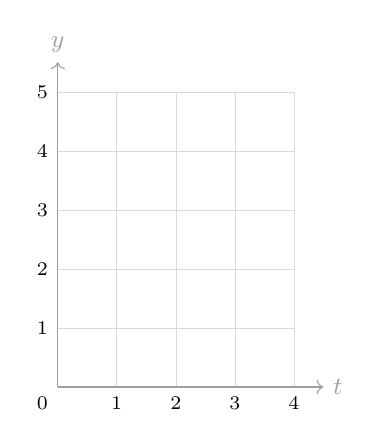
\begin{tikzpicture}[scale=0.75]
  \draw[step=1,gray!30,very thin] (0,0) grid (4,5);
  \draw[axisline] (0,0) -- (4.5,0) node[right,font=\small]{$t$};
  \draw[axisline] (0,0) -- (0,5.5) node[above,font=\small]{$y$};
  \foreach \i in {1,...,4}
    \node[below,font=\scriptsize] at (\i,0) {$\i$};
  \foreach \i in {1,...,5}
    \node[left,font=\scriptsize]  at (0,\i) {$\i$};
  \node[below left,font=\scriptsize] at (0,0) {$0$};
\end{tikzpicture}
\end{minipage}
\par\vspace{0.6cm}
\begin{romparts}[start=3]
  \item Form $\mt{A}\T\mt{A}$ and $\mt{A}\T\vc{b}$, solve the normal equations
        for $\xh$, and write down the best line. Draw it on the axes above.
        \vspace{\stretch{1}}
\end{romparts}
\contd
\begin{romparts}[resume]
  \item Compute the residual $\vc{r}=\vc{b}-\mt{A}\xh$, check that
        $\mt{A}\T\vc{r}=\vc{0}$, and find the sum of the squared errors.
        \vspace{\stretch{1.2}}
  \item Compute $\mt{A}^{+}=(\mt{A}\T\mt{A})^{-1}\mt{A}\T$, and check that
        $\mt{A}^{+}\vc{b}=\xh$.
        \vspace{\stretch{1.2}}
  \item Prove that every least-squares solution $\xh$ of
        $\mt{A}\vc{x}=\vc{b}$ satisfies
        $\norm{\vc{b}}^{2}=\norm{\mt{A}\xh}^{2}+\norm{\vc{b}-\mt{A}\xh}^{2}$.
        Then check it on the data above.
        \hint{The residual $\vc{b}-\mt{A}\xh$ is orthogonal to every column of
        $\mt{A}$, so it is orthogonal to $\mt{A}\xh$.}
        \vspace{\stretch{1.4}}
  \item The single equation $2w_1-w_2+2w_3=18$ is $\mt{C}\vc{w}=18$, with
        $\mt{C}=[\,2,\,-1,\,2\,]\in\R^{1\times3}$ and $\vc{w}\in\R^{3}$. Since
        $\mt{C}$ has independent rows, its pseudo-inverse is
        $\mt{C}^{+}=\mt{C}\T(\mt{C}\mt{C}\T)^{-1}$. Use $\mt{C}^{+}$ to find the
        shortest solution $\vc{w}^{+}$ of $\mt{C}\vc{w}=18$. Compare its length
        with the length of the solution $[\,9,\,0,\,0\,]\T$.
        \vspace{\stretch{1.2}}
\end{romparts}
\end{prob}

\newpage
%------------------------------------------------------------------------------
\begin{prob}[Symmetric and skew-symmetric matrices]
A square matrix $\mt{K}$ is \textbf{skew-symmetric} if $\mt{K}\T=-\mt{K}$.
Prove each statement, naming the law that justifies each step.
\begin{romparts}
  \item For every $\mt{A}\in\R^{n\times n}$, the matrix $\mt{A}+\mt{A}\T$ is
        symmetric and the matrix $\mt{A}-\mt{A}\T$ is skew-symmetric.
        \par\vspace{4.5cm}
  \item The only $n\times n$ matrix that is both symmetric and skew-symmetric is
        the zero matrix.
        \par\vspace{4cm}
  \item For every $\mt{A}\in\R^{m\times n}$, the matrix $\mt{A}\T\mt{A}$ is
        symmetric.
        \par\vspace{3cm}
  \item If $\mt{K}$ is an $n\times n$ skew-symmetric matrix and $n$ is odd, then
        $\det\mt{K}=0$.
        \hint{Compute $\det(\mt{K}\T)$ in two ways.}
        \vfill
\end{romparts}
\end{prob}

\newpage
%------------------------------------------------------------------------------
\begin{prob}[Matrix algebra]
\begin{romparts}
  \item Let $\mt{A}$ and $\mt{B}$ be $n\times n$ matrices. Prove that
        \[
          (\mt{A}+\mt{B})^{2}=\mt{A}^{2}+\mt{A}\mt{B}+\mt{B}\mt{A}+\mt{B}^{2},
        \]
        naming the law used at each step. Then prove that
        $(\mt{A}+\mt{B})^{2}=\mt{A}^{2}+2\mt{A}\mt{B}+\mt{B}^{2}$ if and only if
        $\mt{A}\mt{B}=\mt{B}\mt{A}$.
        \par\vspace{6cm}
  \item Let $\vc{u},\vc{v}\in\R^{n}$. Prove that
        $\tr(\vc{u}\vc{v}\T)=\vc{v}\T\vc{u}$.
        \vfill
\end{romparts}
\contd
\begin{romparts}[resume]
  \item Let $\mt{U}$ and $\mt{V}$ be upper triangular $n\times n$ matrices.
        Prove that $\mt{U}\mt{V}$ is upper triangular, and that its diagonal
        entries are $(\mt{U}\mt{V})_{ii}=u_{ii}v_{ii}$.
        \hint{For $i>j$, look at each term $u_{ik}v_{kj}$ of
        $(\mt{U}\mt{V})_{ij}=\sum_{k}u_{ik}v_{kj}$. If $k<i$, which factor is
        zero? If $k\ge i$, which factor is zero?}
        \vfill
\end{romparts}
\end{prob}

\newpage
%------------------------------------------------------------------------------
\begin{prob}[Orthogonal matrices and projections]
Recall that a square matrix $\mt{Q}$ is \textbf{orthogonal} if
$\mt{Q}\T\mt{Q}=\mt{Q}\mt{Q}\T=\mt{I}$, and that a square matrix $\mt{P}$ is a
\textbf{projection matrix} if $\mt{P}^{2}=\mt{P}$.
\begin{romparts}
  \item Let $\mt{Q}_1$ and $\mt{Q}_2$ be orthogonal $n\times n$ matrices. Prove
        that $\mt{Q}_1\mt{Q}_2$ is orthogonal.
        \par\vspace{5cm}
  \item Let $\mt{Q}$ be an orthogonal matrix. Prove that $\det\mt{Q}=1$ or
        $\det\mt{Q}=-1$.
        \vfill
\end{romparts}
\contd
\begin{romparts}[resume]
  \item Let $\mt{P}$ be an $n\times n$ projection matrix. Prove that
        $\mt{P}\T$ and $\mt{I}-\mt{P}$ are projection matrices.
        \par\vspace{6cm}
  \item Let $\mt{P}$ be an $n\times n$ projection matrix. Prove that a vector
        $\vc{v}\in\R^{n}$ lies in $\colsp{\mt{P}}$ if and only if
        $\mt{P}\vc{v}=\vc{v}$.
        \vfill
\end{romparts}
\end{prob}

\newpage
%------------------------------------------------------------------------------
\begin{prob}[Null spaces, column spaces, and inverses]
\begin{romparts}
  \item Let $\mt{A}\in\R^{m\times n}$ and $\mt{B}\in\R^{p\times m}$. Prove that
        $\nullsp{\mt{A}}\subseteq\nullsp{\mt{B}\mt{A}}$. Then prove that if
        $\nullsp{\mt{B}}=\{\vc{0}\}$, then
        $\nullsp{\mt{B}\mt{A}}=\nullsp{\mt{A}}$.
        \par\vspace{6cm}
  \item Let $\mt{A}\in\R^{m\times n}$ and $\mt{B}\in\R^{n\times p}$. Prove that
        $\colsp{\mt{A}\mt{B}}\subseteq\colsp{\mt{A}}$, and deduce that
        $\rank(\mt{A}\mt{B})\le\rank\mt{A}$.
        \vfill
\end{romparts}
\contd
\begin{romparts}[resume]
  \item Let $\mt{A},\mt{B},\mt{C}$ be invertible $n\times n$ matrices. Prove
        that $\mt{A}\mt{B}\mt{C}$ is invertible, with
        $(\mt{A}\mt{B}\mt{C})^{-1}=\mt{C}^{-1}\mt{B}^{-1}\mt{A}^{-1}$.
        \par\vspace{5.5cm}
  \item Let $\mt{A}$ be an $n\times n$ matrix with $\mt{A}^{2}=\mt{0}$. Prove
        that $\mt{A}$ is not invertible, and that $\mt{I}-\mt{A}$ is invertible
        with $(\mt{I}-\mt{A})^{-1}=\mt{I}+\mt{A}$.
        \vfill
\end{romparts}
\end{prob}

\end{document}
